% !TeX root = ../tfg.tex
% !TeX encoding = utf8

\chapter{Resultados}

En este capítulo se presentan los resultados obtenidos. En primer lugar, se analiza cómo el uso del agrupamiento de variables para la generación de subcomponentes en CC mejora el rendimiento, lo que justifica explorar la aplicación de esta técnica en otros algoritmos como SHADE y SHADE-ILS.

En segundo lugar, se realiza una comparación entre SHADE y SHADE-ILS en sus versiones con y sin agrupamiento de variables, evaluando los casos en los que la introducción de esta estrategia ha supuesto una mejora significativa.

\section{Benchmark}

Para comparar el rendimiento de los algoritmos, se ha utilizado el benchmark \textit{CEC 2013 LSGO} \cite{cec_2013_lsgo}, diseñado específicamente para evaluar algoritmos en problemas de alta dimensionalidad. Este benchmark incluye un total de 15 funciones agrupadas en cuatro categorías, que representan diferentes niveles de separabilidad y complejidad en los problemas de optimización. A continuación, se describen las categorías y las funciones correspondientes:

\subsection{Funciones Totalmente Separables}

Estas funciones son completamente separables, es decir, las variables de decisión no presentan interacciones entre sí. Las funciones en esta categoría son:
\begin{itemize}
    \item \textbf{f1:} Función Elíptica
    \item \textbf{f2:} Función Rastrigin
    \item \textbf{f3:} Función Ackley
\end{itemize}

\subsection{Funciones Parcialmente Separables}

Esta categoría incluye funciones que combinan subcomponentes separables y no separables. Se dividen en dos subcategorías:
\begin{itemize}
    \item \textbf{Funciones con un subcomponente separable:}
    \begin{itemize}
        \item \textbf{f4:} Función Elíptica
        \item \textbf{f5:} Función Rastrigin
        \item \textbf{f6:} Función Ackley
        \item \textbf{f7:} Problema de Schwefel 1.2
    \end{itemize}
    \item \textbf{Funciones sin subcomponentes separables:}
    \begin{itemize}
        \item \textbf{f8:} Función Elíptica
        \item \textbf{f9:} Función Rastrigin
        \item \textbf{f10:} Función Ackley
        \item \textbf{f11:} Problema de Schwefel 1.2
    \end{itemize}
\end{itemize}

\subsection{Funciones con Subcomponentes Superpuestos}

En esta categoría, los subcomponentes tienen cierta superposición, lo que introduce dependencias entre ellos. Estas funciones se dividen en dos tipos:
\begin{itemize}
    \item \textbf{Funciones con subcomponentes conformes:} las variables compartidas entre subcomponentes tienen valores óptimos compatibles.
    \begin{itemize}
        \item \textbf{f12:} Función de Rosenbrock
        \item \textbf{f13:} Función de Schwefel con Subcomponentes Superpuestos Conformes
    \end{itemize}
    \item \textbf{Funciones con subcomponentes conflictivos:} las variables compartidas tienen valores óptimos incompatibles, lo que genera conflictos.
    \begin{itemize}
        \item \textbf{f14:} Función de Schwefel con Subcomponentes Superpuestos Conflictivos
    \end{itemize}
\end{itemize}

\subsection{Funciones Totalmente No Separables}

Estas funciones presentan interacciones entre todas las variables de decisión, lo que dificulta considerablemente el proceso de optimización. En esta categoría se encuentra:
\begin{itemize}
    \item \textbf{f15:} Problema de Schwefel 1.2
\end{itemize}	

\section{Resultados obtenidos}

Los algoritmos fueron ejecutados utilizando el benchmark descrito, estableciendo un límite máximo de 3,000,000 evaluaciones de la función objetivo. Para facilitar la comparación de los resultados, se definieron tres hitos (\textit{milestones}) en los que se registró el valor del óptimo alcanzado por cada algoritmo. Los hitos seleccionados son los siguientes:

\begin{itemize}
    \item \textbf{Primer hito:} 120,000 evaluaciones de la función objetivo.
    \item \textbf{Segundo hito:} 600,000 evaluaciones de la función objetivo.
    \item \textbf{Tercer hito:} 3,000,000 evaluaciones de la función objetivo (resultado final).
\end{itemize}

Para obtener la comparación de los algoritmos, se ha utilizado la web TACO: Toolkit for Automatic Comparison of Optimizers, que permite comparar y obtener resultados de forma rápida fácil y eficaz.

\subsection{Comparación de los métodos de agrupamiento utilizando DECC}

Para comprobar que aplicar un análisis previo de la estructura del problema mediante agrupamiento diferencial, que permita agrupar las variables que interaccionan para optimizarlas de forma independiente, produce resultados beneficiosos, realizaremos una comparación utilizando DECC. Para ello, compararemos los resultados obtenidos en el benchmark por DECC, DECC-ERDG y DECC-DG2.

Observando los resultados obtenidos \ref{tab:resultados_DECC_1} \ref{tab:resultados_DECC_2} \ref{tab:resultados_DECC_3}, podemos concluir que incorporar ERDG para descomponer los problemas del benchmark en subproblemas y luego aplicar Cooperative Coevolution es una estrategia fructífera. Los resultados muestran que DECC-ERDG supera consistentemente a DECC, logrando mejores resultados incluso desde las primeras iteraciones. Esta mejora es particularmente notable en funciones no separables, funciones con componentes superpuestos, funciones parcialmente separables con subcomponentes no separables, como las funciones de tipo Ackley y Schwefel, donde la identificación adecuada de las interacciones entre variables marca una gran diferencia.

Sin embargo, la incorporación de DG2 no ha resultado en mejoras. Por el contrario, ha supuesto una pérdida de rendimiento significativa en comparación con el algoritmo original. Esto puede atribuirse al elevado costo computacional de la estrategia DG2, que consume una gran cantidad de evaluaciones de la función objetivo (500,500 evaluaciones, un sexto del total permitido) únicamente en el proceso de creación de los grupos, dejando menos recursos disponibles para la parte de optimización.

Para realizar esta comparativa, he modificado la versión de DECC implementada por \citeauthor{moesioDECC}, disponible en \cite{moesioDECC}. Esta implementación en Python proporciona una base sólida para experimentar con diferentes métodos de agrupamiento y estrategias de optimización, lo que ha permitido incorporar tanto ERDG como DG2 para su evaluación en el benchmark utilizado.


\subsection{Justificación del éxito de ERDG frente a DG2}

El éxito de ERDG frente a DG2 radica en su eficiencia en el uso de las evaluaciones de la función objetivo. Mientras que DG2 dedica una cantidad considerable de evaluaciones a descomponer los problemas en subcomponentes, ERDG logra realizar esta tarea de manera mucho más eficiente, utilizando un número reducido de evaluaciones. Esto permite a ERDG reservar la mayoría de los recursos disponibles para la optimización, lo que se traduce en un mejor rendimiento global. En la tabla \ref{tab:comparacion_agrupamiento} podemos ver una comparación del número de evaluaciones utilizado por cada algoritmo para descomponer cada problema.

En términos específicos:
\begin{itemize}
\item \textbf{ERDG:} Utiliza una fracción mucho menor de las evaluaciones totales para el análisis de agrupamiento, dejando entre el 90\% y el 99\% del presupuesto para la optimización.
\item \textbf{DG2:} Consume 500,501 evaluaciones exclusivamente en el proceso de agrupamiento, lo que representa aproximadamente un sexto del presupuesto total, reduciendo significativamente las iteraciones disponibles para la optimización.
\end{itemize}

La comparación directa de las evaluaciones utilizadas y los resultados obtenidos en el benchmark refuerza la conclusión de que el equilibrio entre el costo del agrupamiento y el presupuesto de optimización es crucial para el éxito. ERDG logra este equilibrio, mientras que DG2 falla en este aspecto, lo que explica la diferencia de rendimiento observada.

\subsection{Comparación de SHADE y SHADE-ILS con y sin agrupamiento}

Una vez confirmada la eficacia de ERDG, queremos comprobar si puede ser efectiva en algoritmos que no usen coevolución cooperativa. Especialmente estamos interesados en comprobar si hibridar esta técnica con algoritmos pensados directamente para al alta dimensionalidad como SHADE-ILS tiene o no beneficios.

Observando los resultados (tablas \ref{tab:resultados_erdg_shade_1} \ref{tab:resultados_erdg_shade_2} \ref{tab:resultados_erdg_shade_3}) podemos concluir que en general aplicar agrupamiento de variables no reporta buenos resultados al combinarlos con SHADE y SHADE-ILS, en algunos casos siendo contraproducente. Sin embargo, existen ciertos casos donde se puede observar una ligera mejora.

En el caso de funciones no separables (F15) cuando el número de evaluaciones es bajo, ERDG-SHADE obtiene mejores resultados que SHADE, de forma que podemos concluir que en problemas no separables donde se requiera una respuesta rápida, puede ser beneficioso incorporar ERDG a SHADE. Por otra parte, si tenemos más tiempo, siempre será más beneficioso incorporar búsqueda local, ya que SHADE-ILS  obtiene consistentemente mejores resultados que ambas versiones de SHADE y solo en unos pocos casos obtiene peores resultados que ERDG-SHADE-ILS. 

Es interesante observar el caso de las funciones F2 y F4, donde ERDG-SHADE-ILS obtiene resultados claramente superiores a SHADE-ILS, lo que nos hace preguntarnos si aún queda algo que podamos hacer para poder aprovechar mejor el agrupamiento de variables. 

	Estudios recientes muestran que dar la misma importancia a cada subgrupo no es una buena estrategia, ya que el aporte de cada subgrupo a la solución puede variar enormemente en función de cada problema. Nuestra estrategia de prioridad ha sido asignar a los grupos de mayor tamaño un mayor número de evaluaciones, lo que parece en general una buena heurística (ver tabla \ref{tab:comparacion_erdg_shadeils}, sin embargo, es una heurística estática, y no se adapta bien a todos los problemas. Analizando las gráficas \ref{fig:comparacion_erdg_shade_ils}, podemos ver que aquí se obtienen mejores resultados sin adaptar el número evaluaciones al número de grupos.
	
	En \cite{CBCC} se propone usar un método de cooperación coevolutiva (CCFR) basado en la contribución que aporta cada subgrupo a la mejora de la función objetivo, de forma similar al método de selección de búsqueda local de SHADE-ILS. De esta forma, siempre se utilizará para optimizar el grupo que mayor mejora obtuvo en la vez anterior, adaptando dinámicamente el grupo que ha de ser optimizado, eligiendo siempre el más prometedor.
	
\begin{table}[h]
\centering
\begin{tabular}{cccc}
\toprule
{} &       DECC &  DECC-ERDG &   DECC-DG2 \\
\midrule
F01  &  1.396e+08 &  \textcolor{blue}{1.335e+08} &  9.143e+11 \\
F02  &  8.335e+02 &  \textcolor{blue}{8.186e+02} &  1.290e+05 \\
F03  &  \textcolor{blue}{2.000e+01} &  2.156e+01 &  2.170e+01 \\
F04  &  8.252e+13 &  \textcolor{blue}{2.783e+13} &  4.220e+14 \\
F05  &  9.172e+07 &  \textcolor{blue}{4.842e+07} &  5.014e+08 \\
F06  &  \textcolor{blue}{1.066e+06} &  \textcolor{blue}{1.066e+06} &  1.069e+06 \\
F07  &  9.182e+16 &  \textcolor{blue}{7.729e+13} &  2.847e+19 \\
F08  &  8.566e+18 &  \textcolor{blue}{1.003e+18} &  2.217e+19 \\
F09  &  1.126e+10 &  \textcolor{blue}{1.698e+09} &  2.419e+10 \\
F10  &  9.553e+07 &  \textcolor{blue}{9.514e+07} &  9.670e+07 \\
F11  &  8.132e+18 &  \textcolor{blue}{4.576e+12} &  1.840e+22 \\
F12  &  \textcolor{blue}{5.483e+09} &  8.020e+11 &  3.002e+13 \\
F13  &  2.031e+19 &  \textcolor{blue}{5.849e+16} &  8.106e+20 \\
F14  &  1.665e+18 &  \textcolor{blue}{7.270e+16} &  1.663e+21 \\
F15  &  3.447e+12 &  \textcolor{blue}{3.963e+11} &  1.621e+12 \\
Best &          2 &         13 &          0 \\
\bottomrule
\end{tabular}
\caption{Resultados obtenidos por DECC, DECC-ERDG y DECC-DG2 en el primer hito}
\label{tab:resultados_DECC_1}
\end{table}

\begin{table}[h]
\centering
\begin{tabular}{cccc}
\toprule
{} &       DECC &  DECC-ERDG &   DECC-DG2 \\
\midrule
F01  &  \textcolor{blue}{1.881e+06} &  1.941e+06 &  4.647e+11 \\
F02  &  5.474e+01 &  \textcolor{blue}{5.323e+01} &  1.280e+05 \\
F03  &  \textcolor{blue}{2.000e+01} &  2.154e+01 &  2.170e+01 \\
F04  &  8.206e+13 &  \textcolor{blue}{1.421e+13} &  9.925e+13 \\
F05  &  9.132e+07 &  \textcolor{blue}{4.672e+07} &  1.133e+08 \\
F06  &  1.065e+06 &  \textcolor{blue}{1.064e+06} &  1.065e+06 \\
F07  &  9.140e+16 &  \textcolor{blue}{1.223e+13} &  1.567e+18 \\
F08  &  8.522e+18 &  \textcolor{blue}{3.349e+17} &  5.065e+18 \\
F09  &  1.126e+10 &  \textcolor{blue}{7.993e+08} &  8.499e+09 \\
F10  &  9.498e+07 &  \textcolor{blue}{9.475e+07} &  9.555e+07 \\
F11  &  8.116e+18 &  \textcolor{blue}{2.098e+11} &  2.006e+20 \\
F12  &  \textcolor{blue}{5.381e+09} &  2.442e+10 &  9.687e+12 \\
F13  &  2.030e+19 &  \textcolor{blue}{2.950e+15} &  1.665e+20 \\
F14  &  1.664e+18 &  \textcolor{blue}{3.586e+16} &  2.475e+19 \\
F15  &  3.447e+12 &  \textcolor{blue}{2.228e+08} &  1.188e+12 \\
Best &          3 &         12 &          0 \\
\bottomrule
\end{tabular}
\caption{Resultados obtenidos por DECC, DECC-ERDG y DECC-DG2 en el segundo hito.}
\label{tab:resultados_DECC_2}
\end{table}

\begin{table}[h]
\centering
\begin{tabular}{cccc}
\toprule
{} &       DECC &  DECC-ERDG &   DECC-DG2 \\
\midrule
F01  &  4.444e-01 &  \textcolor{blue}{3.690e-01} &  4.634e-01 \\
F02  &  1.033e-02 &  \textcolor{blue}{8.605e-03} &  1.047e-02 \\
F03  &  \textcolor{blue}{2.000e+01} &  2.149e+01 &  \textcolor{blue}{2.000e+01} \\
F04  &  8.206e+13 &  \textcolor{blue}{5.140e+12} &  9.823e+13 \\
F05  &  9.130e+07 &  \textcolor{blue}{2.428e+07} &  7.720e+07 \\
F06  &  \textcolor{blue}{1.063e+06} &  \textcolor{blue}{1.063e+06} &  \textcolor{blue}{1.063e+06} \\
F07  &  9.140e+16 &  \textcolor{blue}{2.848e+10} &  1.547e+16 \\
F08  &  8.522e+18 &  \textcolor{blue}{1.152e+17} &  5.042e+18 \\
F09  &  1.126e+10 &  \textcolor{blue}{6.247e+08} &  6.878e+09 \\
F10  &  9.448e+07 &  \textcolor{blue}{9.463e+07} &  9.480e+07 \\
F11  &  8.116e+18 &  \textcolor{blue}{1.201e+10} &  8.487e+18 \\
F12  &  5.377e+09 &  \textcolor{blue}{1.300e+06} &  5.527e+09 \\
F13  &  2.030e+19 &  \textcolor{blue}{3.211e+13} &  2.089e+18 \\
F14  &  1.664e+18 &  \textcolor{blue}{8.510e+14} &  1.540e+19 \\
F15  &  3.447e+12 &  \textcolor{blue}{1.480e+08} &  1.188e+12 \\
Best &          2 &         13 &          1 \\
\bottomrule
\end{tabular}
\caption{Resultados obtenidos por DECC, DECC-ERDG y DECC-DG2 en el tercer hito.}
\label{tab:resultados_DECC_3}
\end{table}

\begin{table}[h]
\centering
\begin{tabular}{lccc}
\toprule
{} & \textbf{120,000 Evaluaciones} & \textbf{600,000 Evaluaciones} & \textbf{3,000,000 Evaluaciones} \\
\midrule
DECC      &  2 &  3 &  2 \\
DECC-ERDG &  13 &  12 &  13 \\
DECC-DG2  &  0 &  0 &  1 \\
\bottomrule
\end{tabular}
\caption{Número de funciones en las que cada algoritmo obtuvo el mejor resultado en los tres hitos evaluados.}
\label{tab:resultados_comparativos_hitos}
\end{table}

\begin{table}[h]
\centering
\begin{tabular}{ccc}
\toprule
\textbf{Función} & \textbf{Evaluaciones ERDG} & \textbf{Evaluaciones DG2}\\
\midrule
F01  &  2998  &  500501 \\
F02  &  2998  &  500501 \\
F03  &  3996  &  500501 \\
F04  &  5332  &  500501 \\
F05  &  5395  &  500501 \\
F06  &  5901  &  500501 \\
F07  &  5562  &  500501 \\
F08  &  8449  &  500501 \\
F09  &  8780  &  500501 \\
F10 &  8806  &  500501 \\
F11 &  9202  &  500501 \\
F12 &  30440 &  500501 \\
F13 &  7774  &  500501 \\
F14 &  8867  &  500501 \\
F15 &  3996  &  500501 \\
\bottomrule
\end{tabular}
\caption{Comparación del número de evaluaciones utilizadas por ERDG y DG2 en cada función del benchmark.}
\label{tab:comparacion_agrupamiento}
\end{table}

\begin{table}[h]
\centering
\begin{tabular}{ccccc}
\toprule
{} &  \textbf{ERDG-SHADE} & \textbf{ERDG-SHADE-ILS} & \textbf{SHADE} & \textbf{SHADE-ILS} \\
\midrule
F01  &  3.569e+11 &    3.582e+11 &  3.538e+08 &  \textcolor{blue}{2.467e+06} \\
F02  &  1.142e+05 &    1.076e+05 &  1.438e+04 &  \textcolor{blue}{2.878e+03} \\
F03  &  2.140e+01 &    2.014e+01 &  2.140e+01 &  \textcolor{blue}{2.013e+01} \\
F04  &  2.904e+13 &    1.535e+13 &  7.098e+10 &  \textcolor{blue}{3.508e+10} \\
F05  &  6.966e+07 &    9.795e+06 &  4.934e+06 &  \textcolor{blue}{2.354e+06} \\
F06  &  1.072e+06 &    1.072e+06 &  1.063e+06 &  \textcolor{blue}{1.052e+06} \\
F07  &  2.586e+15 &    4.227e+11 &  \textcolor{blue}{2.986e+08} &  6.762e+08 \\
F08  &  1.547e+18 &    6.609e+15 &  \textcolor{blue}{6.685e+13} &  2.188e+14 \\
F09  &  5.702e+09 &    5.693e+09 &  4.480e+08 &  \textcolor{blue}{2.667e+08} \\
F10  &  9.638e+07 &    9.638e+07 &  9.466e+07 &  \textcolor{blue}{9.398e+07} \\
F11  &  6.447e+17 &    1.168e+17 &  \textcolor{blue}{3.699e+09} &  1.965e+10 \\
F12  &  5.478e+09 &    5.688e+06 &  5.122e+09 &  \textcolor{blue}{3.535e+06} \\
F13  &  7.378e+09 &    1.254e+10 &  \textcolor{blue}{8.503e+09} &  1.122e+10 \\
F14  &  \textcolor{blue}{4.751e+10} &    5.385e+10 &  4.893e+10 &  1.086e+11 \\
F15  &  \textcolor{blue}{2.175e+07} &    4.602e+07 &  2.188e+07 &  4.566e+07 \\
Best &          3 &            0 &          3 &         \textcolor{blue}{9} \\
\bottomrule
\end{tabular}
\caption{Resultados obtenidos por ERDG-SHADE, ERDG-SHADE-ILS, SHADE y SHADE-ILS en el primer hito.}
\label{tab:resultados_erdg_shade_1}
\end{table}

\begin{table}[h]
\centering
\begin{tabular}{ccccc}
\toprule
{} &  \textbf{ERDG-SHADE} & \textbf{ERDG-SHADE-ILS} & \textbf{SHADE} & \textbf{SHADE-ILS} \\
\midrule
F01  &  3.569e+11 &    9.222e+09 &  4.345e+07 &  \textcolor{blue}{3.567e-23} \\
F02  &  1.093e+05 &    7.202e+03 &  1.359e+04 &  \textcolor{blue}{2.031e+03} \\
F03  &  2.116e+01 &    \textcolor{blue}{2.005e+01} &  2.116e+01 &  2.007e+01 \\
F04  &  2.705e+13 &    9.011e+10 &  8.216e+09 &  \textcolor{blue}{4.656e+09} \\
F05  &  2.048e+07 &    7.854e+06 &  2.822e+06 &  \textcolor{blue}{1.746e+06} \\
F06  &  1.072e+06 &    1.065e+06 &  1.060e+06 &  \textcolor{blue}{1.045e+06} \\
F07  &  1.390e+14 &    1.055e+09 &  \textcolor{blue}{2.050e+07} &  2.415e+07 \\
F08  &  1.476e+17 &    2.705e+14 &  \textcolor{blue}{4.149e+12} &  1.565e+13 \\
F09  &  5.696e+09 &    5.362e+08 &  3.105e+08 &  \textcolor{blue}{2.161e+08} \\
F10  &  9.638e+07 &    9.529e+07 &  9.406e+07 &  \textcolor{blue}{9.323e+07} \\
F11  &  6.446e+17 &    3.934e+10 &  6.198e+08 &  \textcolor{blue}{4.628e+08} \\
F12  &  2.192e+08 &    2.333e+03 &  2.408e+08 &  \textcolor{blue}{2.193e+03} \\
F13  &  \textcolor{blue}{1.011e+09} &    1.176e+09 &  1.107e+09 &  1.013e+09 \\
F14  &  3.528e+09 &    1.635e+09 &  \textcolor{blue}{1.525e+09} &  2.107e+09 \\
F15  &  6.329e+06 &    6.131e+06 &  6.129e+06 &  \textcolor{blue}{5.921e+06} \\
Best &          1 &            1 &          3 &         \textcolor{blue}{10} \\
\bottomrule
\end{tabular}
\caption{Resultados obtenidos por ERDG-SHADE, ERDG-SHADE-ILS, SHADE y SHADE-ILS en el segundo hito.}
\label{tab:resultados_erdg_shade_2}
\end{table}

\begin{table}[h]
\centering
\begin{tabular}{ccccc}
\toprule
{} &  \textbf{ERDG-SHADE} & \textbf{ERDG-SHADE-ILS} & \textbf{SHADE} & \textbf{SHADE-ILS} \\
\midrule
F01  &  2.514e+11 &    1.757e+04 &  9.882e+06 &  \textcolor{blue}{7.658e-24} \\
F02  &  2.450e+04 &    \textcolor{blue}{2.292e+02} &  1.347e+04 &  1.690e+03 \\
F03  &  2.051e+01 &    \textcolor{blue}{2.004e+01} &  2.045e+01 &  \textcolor{blue}{2.004e+01} \\
F04  &  2.511e+10 &    \textcolor{blue}{4.844e+08} &  1.568e+09 &  1.297e+09 \\
F05  &  9.501e+06 &    3.462e+06 &  1.954e+06 &  \textcolor{blue}{1.419e+06} \\
F06  &  1.060e+06 &    1.059e+06 &  1.056e+06 &  \textcolor{blue}{1.040e+06} \\
F07  &  5.376e+08 &    2.524e+04 &  5.604e+06 &  \textcolor{blue}{1.490e+03} \\
F08  &  1.053e+14 &    1.971e+13 &  \textcolor{blue}{1.933e+11} &  2.784e+12 \\
F09  &  7.001e+08 &    2.291e+08 &  2.538e+08 &  \textcolor{blue}{1.817e+08} \\
F10  &  9.454e+07 &    9.465e+07 &  9.326e+07 &  \textcolor{blue}{9.272e+07} \\
F11  &  7.148e+13 &    1.614e+07 &  9.612e+07 &  \textcolor{blue}{1.423e+06} \\
F12  &  8.737e+07 &    \textcolor{blue}{1.526e+03} &  1.792e+07 &  1.708e+03 \\
F13  &  1.075e+08 &    2.301e+06 &  1.180e+08 &  \textcolor{blue}{4.261e+05} \\
F14  &  2.101e+09 &    2.478e+07 &  2.024e+08 &  \textcolor{blue}{1.088e+07} \\
F15  &  1.943e+06 &    1.129e+06 &  1.767e+06 &  \textcolor{blue}{1.089e+06} \\
Best &          0 &            4 &          1 &         \textcolor{blue}{10} \\
\bottomrule
\end{tabular}
\caption{Resultados obtenidos por ERDG-SHADE, ERDG-SHADE-ILS, SHADE y SHADE-ILS en el tercer hito.}
\label{tab:resultados_erdg_shade_3}
\end{table}

\begin{table}[h]
\centering

\begin{tabular}{lccc}
\toprule
\textbf{Algoritmo} & \textbf{120,000 Evaluaciones} & \textbf{600,000 Evaluaciones} & \textbf{3,000,000 Evaluaciones} \\
\midrule
\textbf{ERDGshade}    &  3 &  1 &  0 \\
\textbf{ERDGshadeils} &  0 &  1 &  4 \\
\textbf{shade}        &  3 &  3 &  1 \\
\textbf{shadeils}     &  9 &  10 &  10 \\
\bottomrule
\end{tabular}
\caption{Número de funciones en las que cada algoritmo obtuvo el mejor resultado en los tres hitos evaluados.}
\label{tab:resultados_comparativos_erdg_shade}
\end{table}

\begin{table}[h]
\centering
\begin{tabular}{lcc}
\toprule
\textbf{Función} & \textbf{ERDG-SHADE-ILS ponderado} & \textbf{ERDG-SHADE-ILS sin ponderar} \\
\midrule
F01  &  \textcolor{blue}{1.757e+04} &  3.247e+11 \\
F02  &  \textcolor{blue}{2.292e+02} &  9.691e+04 \\
F03  &  2.004e+01 &  2.004e+01 \\
F04  &  \textcolor{blue}{4.844e+08} &  2.159e+11 \\
F05  &  \textcolor{blue}{3.462e+06} &  9.698e+06 \\
F06  &  1.059e+06 &  \textcolor{blue}{1.041e+06} \\
F07  &  \textcolor{blue}{2.524e+04} &  1.289e+09 \\
F08  &  \textcolor{blue}{1.971e+13} &  2.126e+14 \\
F09  &  \textcolor{blue}{2.291e+08} &  3.649e+08 \\
F10  &  9.465e+07 &  \textcolor{blue}{9.203e+07} \\
F11  &  \textcolor{blue}{1.614e+07} &  2.139e+08 \\
F12  &  \textcolor{blue}{1.526e+03} &  1.746e+03 \\
F13  &  2.301e+06 &  \textcolor{blue}{2.233e+06} \\
F14  &  \textcolor{blue}{2.478e+07} &  6.008e+10 \\
F15  &  \textcolor{blue}{1.129e+06} &  1.185e+06 \\
Best &           \textcolor{blue}{11} &              4 \\
\bottomrule
\end{tabular}
\caption{Comparación entre ERDG-SHADE-ILS dando la misma importancia a los grupos y ponderando en función del tamaño en los resultados obtenidos para cada función del benchmark.}
\label{tab:comparacion_erdg_shadeils}
\end{table}

\begin{figure}[h]
\centering
\begin{subfigure}{0.8\textwidth}
    \centering
    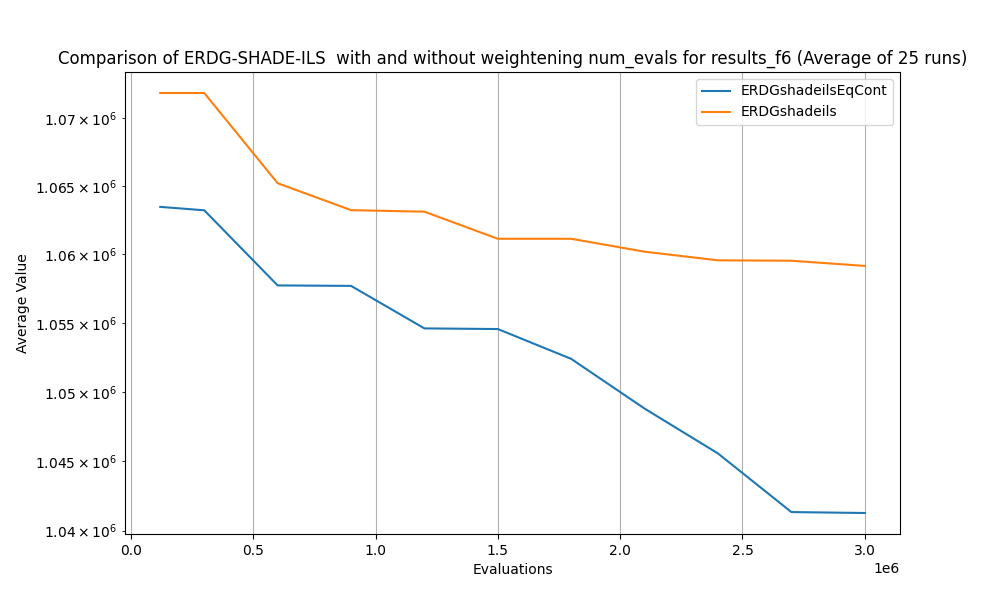
\includegraphics[width=\textwidth]{images/comparison_cont_f6.png} % Reemplaza "comparison_cont_f6.png" con el nombre de tu archivo
    \caption{Comparación para F6}
\end{subfigure}
\vspace{0.5cm} % Espacio entre las imágenes
\begin{subfigure}{0.8\textwidth}
    \centering
    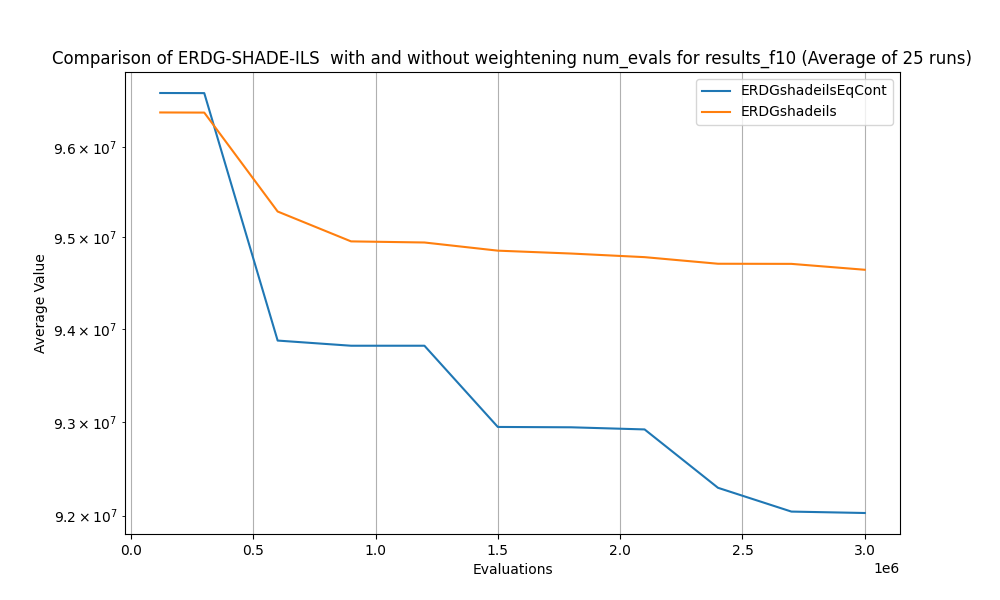
\includegraphics[width=\textwidth]{images/comparison_cont_f10.png} % Reemplaza "comparison_cont_f10.png" con el nombre de tu archivo
    \caption{Comparación para F10}
\end{subfigure}
\caption{Comparación políticas asignación de evaluaciones ERDG-SHADE-ILS.}
\label{fig:comparacion_erdg_shade_ils}
\end{figure}



\endinput
%--------------------------------------------------------------------
% FIN DEL CAPÍTULO. 
%--------------------------------------------------------------------
Comparar el algoritmo clásico con DG2 ERDG y H con CC
Comparar SHADE y SHADEILS con y sin ERDG en cada uno de los tipos